\documentclass[9pt,a4paper]{extarticle}
\usepackage[a4paper,margin=1.55cm]{geometry}
\usepackage[utf8]{inputenc}
\usepackage[T1]{fontenc}
\usepackage{helvet}
\renewcommand{\familydefault}{\sfdefault}
\DeclareUnicodeCharacter{00D7}{\ensuremath{\times}}
\DeclareUnicodeCharacter{2013}{\textendash}
\DeclareUnicodeCharacter{201C}{``}
\DeclareUnicodeCharacter{201D}{''}
\DeclareUnicodeCharacter{2192}{\ensuremath{\rightarrow}}
\usepackage{graphicx}
\usepackage{enumitem}
\usepackage{microtype}
\usepackage{parskip}
\setlength{\parindent}{0pt}
\setlength{\parskip}{4pt}
\pagestyle{empty}
\setlist[itemize]{leftmargin=1.5em,itemsep=1.2pt,topsep=2pt,parsep=0pt,partopsep=0pt,label=\textbullet}
\newcommand{\Sec}[1]{\vspace{2pt}\noindent\textbf{#1}\par\vspace{2pt}}
\newcommand{\Sub}[1]{\vspace{2pt}\noindent\textbf{#1}\par\vspace{1pt}}
\begin{document}
\fontsize{8.6}{10.2}\selectfont

Faculty of Electrical Engineering - University of Sarajevo

Mentor Prof. dr. Izudin Džafić

Student Almir Mustafić

\vfill
\begin{center}
{\fontsize{17}{20}\selectfont\textbf{GaussNewtonFit}}\\[8pt]
{\fontsize{11.5}{14}\selectfont\textbf{Gauss-Newton Method for Nonlinear Parameter Estimation}}\\[2pt]
{\fontsize{11.5}{14}\selectfont\textbf{and Model Fitting}}
\end{center}
\vfill
\newpage

\Sec{Executive Summary}
GaussNewtonFit is a C++14 system for nonlinear least-squares parameter estimation. The system implements Gauss\mbox{-}Newton and full Newton-Raphson solvers. It compares both methods under the same models, datasets, noise levels, initial parameter values, and stopping criteria.

The system generates synthetic data for exponential decay, logistic growth, and sinusoidal models. Users can run a fit from the desktop interface and inspect the fitted curve, residual history, estimated parameters, and execution log. The \mbox{command-line} test harness also validates analytical derivatives and runs a 36-experiment comparison.

The project studies solver behavior under controlled conditions. The comparison measures convergence, failure, iteration count, residual norm, execution time, and parameter error.

\Sec{1. About the Project}
GaussNewtonFit solves nonlinear parameter estimation problems by minimizing least-squares residuals. The project uses two optimization methods for the same fitting tasks. This setup isolates differences between Gauss-Newton and full Newton.
\begin{itemize}
\item The system fits an exponential decay model with two parameters.
\item The system fits a logistic growth model with three parameters.
\item The system fits a sinusoidal model with three parameters.
\item The system generates synthetic data with configurable Gaussian noise.
\item The system records the residual norm during every solver iteration.
\item The system exports experiment results and run reports to files.
\end{itemize}
\newpage

\Sec{2. System Architecture Overview}
GaussNewtonFit separates data generation, model evaluation, solver logic, testing, visualization, and export functions.
\begin{itemize}
\item The data generator creates synthetic observations for the selected model.
\item The model layer evaluates predictions and analytical derivatives.
\item The solver layer runs Gauss-Newton or full Newton.
\item The test harness checks derivatives and runs batch experiments.
\item The GUI shows the model fit and residual history.
\item The export layer writes logs, reports, CSV files, and plot states.
\end{itemize}

\Sec{3. Technology Stack}
\begin{itemize}
\item C++14 implements the models, solvers, tests, file export, and application logic.
\item CMake manages the project build.
\item The Matrix library performs matrix operations and solves linear systems.
\item natGUI provides the desktop interface.
\item natPlot renders the model-fit and convergence plots.
\item The C++ standard library provides random number generation, timing, mathematical functions, and file operations.
\end{itemize}

\Sec{4. Models and Datasets}
The project uses synthetic datasets only. Each dataset contains 10 equidistant sample points on the interval from 0 to 5. The experiments use Gaussian noise levels of 0.00, 0.05, and 0.20 with a fixed random seed of 42.
\begin{itemize}
\item The exponential dataset uses y = 2.0 exp(-0.3 t) + e. The ground-truth parameters are 2.0 and 0.3.
\item The logistic dataset uses y = 10.0 / (1 + exp(-1.5(t - 2.5))) + e. The ground-truth parameters are 10.0, 1.5, and 2.5.
\item The sinusoidal dataset uses y = 3.0 sin(2.0 t + 0.5) + e. The ground-truth parameters are 3.0, 2.0, and 0.5.
\end{itemize}
\newpage

\Sec{5. Optimization Methods}
GaussNewtonFit implements two solvers for the same nonlinear least-squares objective.

\Sub{5.1 Gauss-Newton}
Gauss-Newton uses first-order derivatives. The method forms the matrix J\textasciicircum T J and solves a linear system for the parameter update. The method does not use second-order residual derivatives.

The solver computes the residual vector and the Jacobian at the current parameter estimate. It solves the normal equations and updates the parameter vector. It repeats this process until a stopping condition is met.

\Sub{5.2 Full Newton-Raphson}
Full Newton uses first-order and second-order derivatives. The method forms the exact least-squares Hessian by combining J\textasciicircum T J with the residual-weighted Hessians of the model residuals.

The solver computes the residual vector, Jacobian, and residual Hessians at the current parameter estimate. It solves the resulting linear system and updates the parameter vector. It repeats this process until a stopping condition is met.

\Sub{5.3 Shared Stopping Criteria}
Both solvers use the same stopping rules. A run succeeds when the maximum parameter step falls below the tolerance or when the residual norm falls below the tolerance. A run is marked as failed when the maximum iteration count is reached without meeting the required residual condition.

\Sec{6. Analytical Derivatives and Validation}
The system implements analytical Jacobians for all three models. Full Newton also uses analytical residual Hessians for every data point.

The test suite checks these derivatives against central finite differences. The derivative check uses a perturbation of 1e-6. The accepted Jacobian error is below 1e-4. The accepted Hessian error is below 3e-3.
\newpage

\Sec{7. Experiment Design}
The automated comparison runs 36 experiments. The grid combines three models, two solvers, three noise levels, and two initial parameter offsets.
\begin{itemize}
\item The project tests the exponential, logistic, and sinusoidal models.
\item The project tests Gauss-Newton and full Newton.
\item The project tests noise levels of 0.00, 0.05, and 0.20.
\item The project tests initial parameter offsets of 0.05 and 1.0.
\end{itemize}
The system records the iteration count, final residual norm, estimated parameters, parameter error, execution time, and failure status for each run.

\Sec{8. Key Results}
Both solvers converge from close initial values across all three models. These runs usually finish within 3 to 7 iterations and reach similar parameter accuracy.

The exponential model separates the methods under distant initialization. Gauss-Newton converges in about 7 to 11 iterations. Full Newton reaches the 50-iteration limit and produces a large parameter error in the tested configuration.

The logistic model produces the opposite result under distant initialization. Gauss-Newton stalls in the flat saturation region and produces large parameter errors. Full Newton converges in about 7 to 8 iterations because the second-order term provides curvature information.

The sinusoidal model remains sensitive to the initial parameter values. Both methods can converge to incorrect phase or frequency regions when the initial values are not suitable.

Higher noise increases the final residual norm because the fitted model cannot remove the added measurement noise.
\newpage

\Sec{9. Inputs and Outputs}
The application accepts a model selection, a solver selection, a noise level, and initial parameter values. The command-line tests also use a maximum iteration count, a tolerance, and a fixed random seed.

The application returns an estimated parameter vector and a residual history. It also reports the iteration count, final residual norm, execution time, and failure status.

The program writes several result files during testing and export.
\begin{itemize}
\item The files exponential.csv, logistic.csv, and sinusoidal.csv store generated datasets.
\item The file comparison\_results.csv stores the full experiment grid.
\item The file comparison\_summary.csv stores side-by-side solver comparisons.
\item The file fit\_log.txt stores the GUI execution history.
\item The file run\_export.txt stores a formatted report for one run.
\item The files fit\_plot.xml and convergence\_plot.xml store plot states.
\end{itemize}

\Sec{10. Target Users}
\begin{itemize}
\item Students can use the project to study nonlinear least-squares methods.
\item Instructors can use the project to demonstrate convergence and failure behavior.
\item Researchers can use the project to compare solver behavior under controlled conditions.
\item Engineers can use the project to test nonlinear model fitting.
\end{itemize}
\newpage

\Sec{11. Existing Alternatives}
Several existing libraries and applications solve nonlinear least-squares problems.
\begin{itemize}
\item SciPy provides nonlinear least-squares and curve-fitting methods in Python.
\item Ceres Solver provides nonlinear optimization tools in C++.
\item GNU Scientific Library provides numerical fitting and optimization methods in C.
\item MATLAB Optimization Toolbox provides nonlinear model-fitting functions.
\end{itemize}

\Sec{12. Why This Project Matters}
GaussNewtonFit focuses on the direct comparison of Gauss-Newton and full Newton. Both solvers use the same models, data, matrix operations, stopping rules, and result metrics.

The project exposes the mathematical difference between the two methods. Gauss-Newton uses J\textasciicircum T J. Full Newton adds the residual-weighted second-derivative term.

The project also shows failure cases that general-purpose libraries may hide through damping, trust regions, or line\mbox{-}search procedures. The experiments therefore show how the base methods behave before those additional mechanisms are added.

The code uses analytical derivatives for the tested models. The test harness checks those derivatives with finite differences before running the solver comparisons.
\newpage

\Sec{13. Graphical User Interface}
The desktop interface lets the user select a model and an optimization method. The user sets the noise level and the initial parameter values before running the fit.

The left plot shows the generated data and the fitted model. The right plot shows the residual norm by iteration. The status line reports the iteration count and final residual norm. The execution log lists recent runs. The export control writes the current log to a file.

\vspace{12pt}
\begin{center}
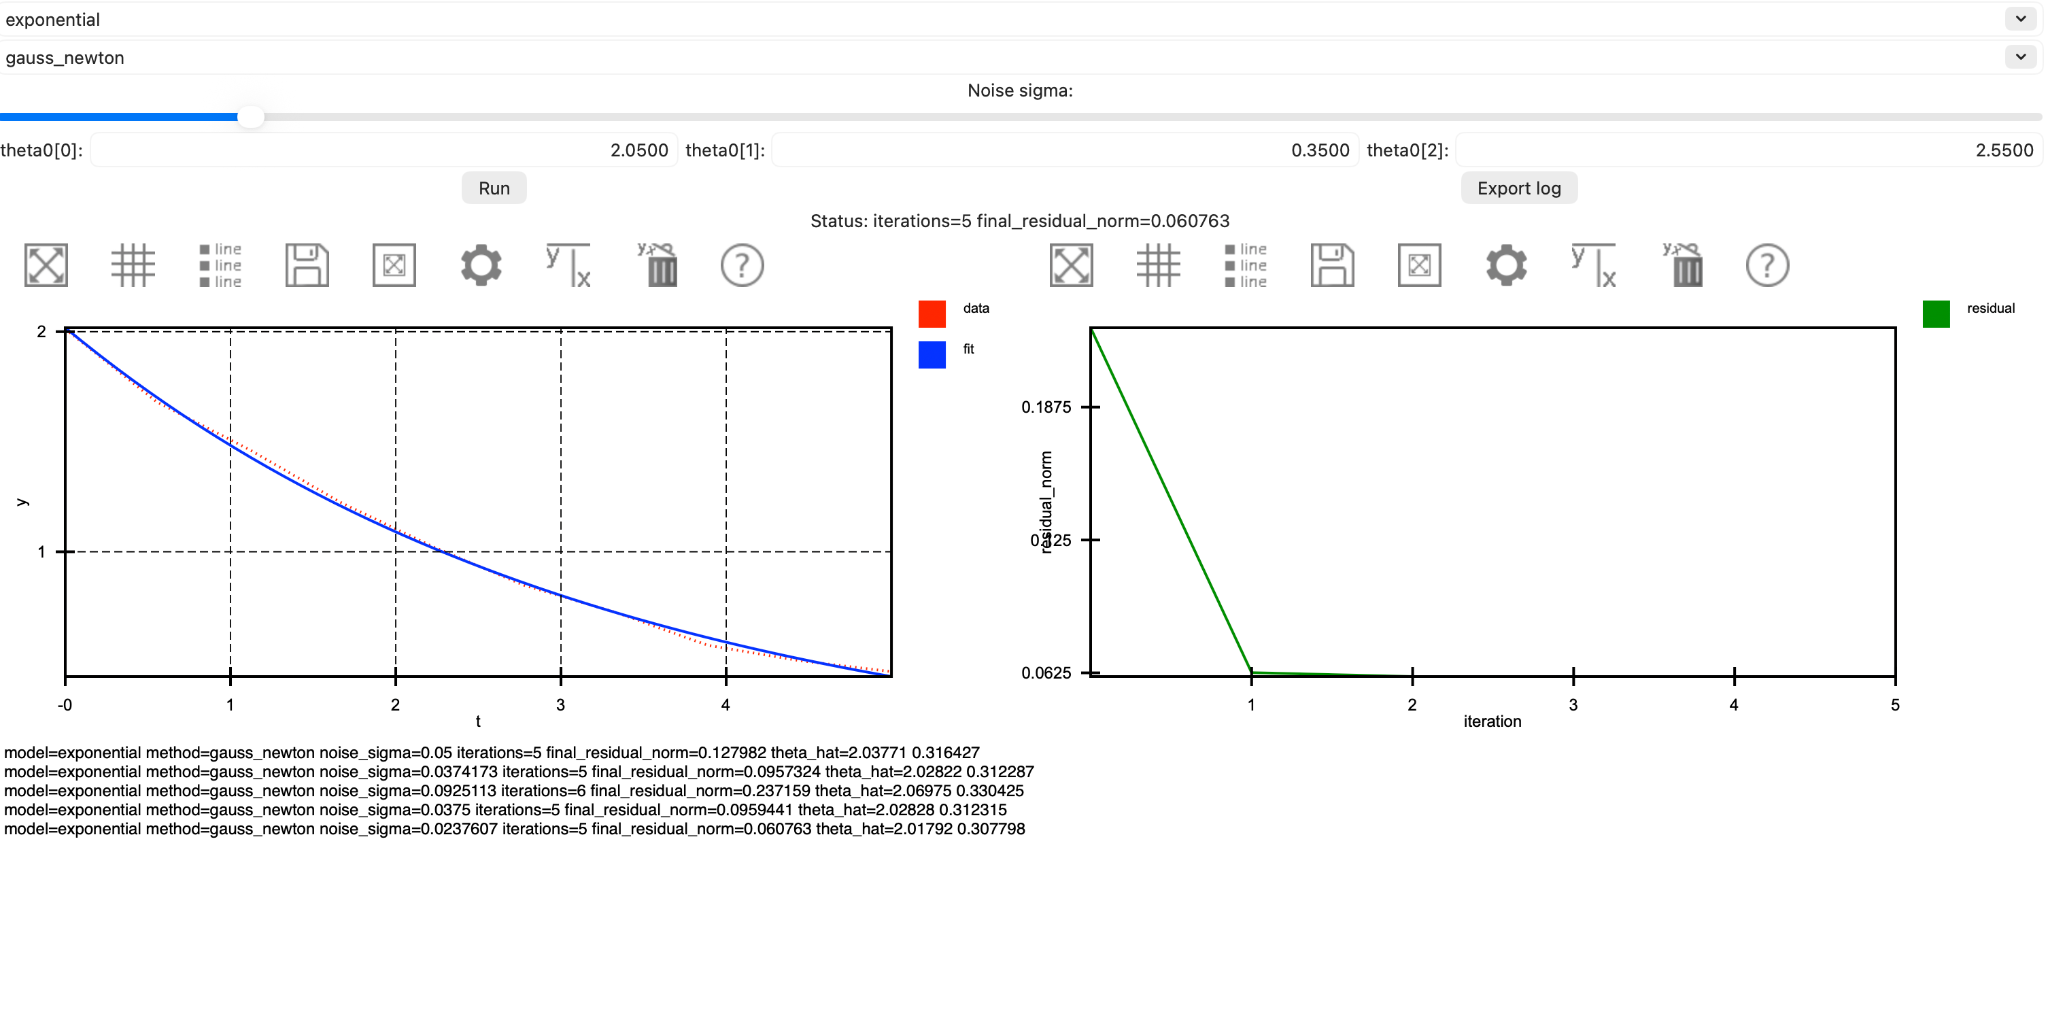
\includegraphics[width=0.88\textwidth]{assets/gn-000.png}\\[5pt]
Figure 1 - GaussNewtonFit desktop interface
\end{center}
\newpage

\Sec{14. Current Limitations}
\begin{itemize}
\item The system uses synthetic datasets and does not import measured datasets through the GUI.
\item The GUI provides three parameter input fields and therefore limits interactive use to models with up to three parameters.
\item The solvers use unweighted least squares even though the dataset structure stores noise information.
\item The solvers use full update steps without damping or line search.
\item The linear solver marks the run as failed when the system matrix becomes singular or poorly conditioned.
\end{itemize}

\Sec{15. Future Work}
\begin{itemize}
\item The project can add CSV or TSV import for measured datasets.
\item The project can add weighted least squares.
\item The project can add Levenberg-Marquardt damping or trust-region control.
\item The project can add covariance estimates, parameter standard errors, confidence intervals, and R-squared values.
\item The GUI can support models with more than three parameters.
\item The application can add support for user-defined model equations.
\end{itemize}

\Sec{16. Conclusion}
GaussNewtonFit implements Gauss-Newton and full Newton for the same nonlinear fitting tasks. The project compares how both methods respond to noise and initial parameter values. The results show that neither method performs best in every tested case. The application combines the solver comparison with derivative checks, batch experiments, plots, and file export.

\end{document}
